Toda esta sección queda anémica y siento que dice cosas o no muy interesantes o de las que no tenemos tanto que decir.
Me parece más bien un punteo de temas que se podrían mencionar que un draft de una versión a incluir verdaderamente.

\section{Algoritmo clásico}
Para implementar el algoritmo clásico de construcción de EPAs necesitamos lo siguiente:
\begin{itemize}
    \item Obtener la lista de métodos y de precondiciones de un contrato
    \item Poder definir estados de un contrato que garantizen el invariante
    \item Poder ejecutar los métodos y precondiciones del contrato de manera aislada
    \item Poder ejecutar el invariante del contrato de manera aislada
    \item Realizar consultas sobre el resultado de la ejecución de estos
\end{itemize}
Afortunadamente, la API de Manticore de los contratos inteligentes deployeados ofrece acceso a la lista de sus métodos de manera nativa.
Sin embargo, dado que la abstracción de estos es a nivel bytecode, no resultaba posible extraer de manera automática las precondiciones.
Por otro lado, como mencionamos en la sección \ref{sec:api-manticore} la API programable sólo nos permite generar estados a partir de la ejecución directa de métodos a instancias desde el constructor inicial.
Estas dos limitaciones significaron que tuvimos que introducir las precondiciones como métodos explícitos a los contratos de manera manual, y que necesitamos introducir alguna forma de simular la ejecución de los métodos en el vacío.

Debido al alcance previsto para la experimentación con la herramienta, y para mantener el tiempo de desarrollo al mínimo, optamos por no automatizar la extracción de precondiciones de los métodos en métodos independientes, sino que se realizó de manera totalmente manual en los contratos con los que experimentamos.
De todas formas, debido a que los contratos inteligentes incluyen sus precondiciones de manera explícita al comienzo de los métodos, esta traducción manual consistió en copiar las secciones relevantes y reemplazar las apariciones de \textcolor{magenta}{\texttt{require}} por \textcolor{magenta}{\texttt{return}}.
Luego, para identificar estos métodos automáticamente desde Manticore, establecimos la convención de nomenclatura de introducirles el sufijo \textcolor{orange}{\texttt{\_precondition}}.
Por ejemplo, el método que implementa la preconidición explícita del método \textcolor{orange}{\texttt{MakeOffer}} se llamaría \textcolor{orange}{\texttt{MakeOffer\_precondition}}.

Para poder emular la ejecución de los métodos de manera aislada, era necesario poder construir dentro de Manticore estados completamente genéricos.
Es decir, obtener valores para las variables de la blockchain y las variables de estado totalmente arbitrarios, que no encontraran restrictos a ser una de las posibles configuraciones resultantes de una secuencia de métodos en particular.
Dado que la API de Manticore sobre los contratos no provee acceso directo a las variables o el storage de los contratos (sólo permite interacturar con los métodos y el estado de la blockchain), decidimos solucionarlo modificando los valores de las variables externamente mediante métodos.
Para esto, también consideramos que lo más veloz en tiempo de desarrollo sería introducir manualmente un método externo, ``\textcolor{orange}{\texttt{setter}}'', al contrato que recibe un parámetro por cada variable de estado en el contrato, y que asigna el valor recibido a esta.
De esta manera, ejecutar \textcolor{orange}{\texttt{setter}} con parámetros simbólicos genera un estado genérico del contrato.

Los estados resultantes de este proceso, sin embargo, al ser totalmente irrestrictos, no garantizaban el cumplimiento del invariante.
Para reintroducir esta propiedad luego de llamar al \textcolor{orange}{\texttt{setter}} del contrato, aprovechamos la interfaz del módulo \texttt{\textbf{smtlib}} de Manticore.
Lo más sencillo fue introducir el invariante como método explícito de manera manual sólo en el código fuente de los contratos.
Luego usamos este método para restringir los estados genéricos sobre su resultado, de manera análoga a como usamos las implementaciones de las precondiciones.
Los invariantes a lo largo del desarrollo fueron producidos de manera manual para cada contrato, razonando artesanalmente sobre las variables de estado del contrato y como sus métodos las modificaban.

\section{Algoritmo alternativo}
Los requisitos para implementar el algoritmo alternativo son muy similares.
Resulta necesario lo siguiente:
\begin{itemize}
    \item Obtener la lista de métodos y de precondiciones de un contrato
    \item Poder ejecutar los métodos y precondiciones del contrato de manera aislada
    \item Realizar consultas sobre el resultado de la ejecución de estos
    \item Poder retroceder pasos en la ejecución del contrato hasta un estado anterior
\end{itemize}
De estos items, notamos que los primeros tres se comparten con el algoritmo clásico y, de hecho, fueron tratados con la mismas soluciones ya descritas.
Sin embargo, la necesidad de poder realizar \textit{rollbacks} en la ejecución del contrato analizado, a pesar de ser deseable en la implementación del algoritmo clásico, era crucial en la implementación del algoritmo alternativo.
Esto es porque en este algoritmo los estados de la EPA se descubren mediante sucesiones crecientes de llamados a métodos.
Si no fuera posible realizar un paso en la EPA, retroceder, y luego realizar otro, significaría que para explorar estados profundos deberíamos levantar una nueva instancia del contrato y repetir la ejecución de los métodos que nos hacen alcanzar el estado cada vez.

Por este motivo, modificamos el módulo \textbf{\texttt{manticorebase}} para permitir retroceder en el historial de transacciones externas del contrato.
Estos cambios, junto con otras pequeñas modificaciones y correcciones de defectos en la herramienta pueden verse en el repositorio \cite{manticore-tiny-changes}.
La implementación de estos dos algoritmos, por su parte, está pública en el repositorio \cite{manticore-predicate-abstraction}.

Otro detalle implementativo que hubo que solucionar en esta etapa surge de una pecularidad de Manticore frente a las variables de tipo \texttt{account} (que representan entidades en la blockchain, sea usuario o contrato) simbólicas.
El problema surgía de que Manticore, al mantener una simulación completa de la blockchain, buscaba resolver estas variables a algún valor que se condijera con una \texttt{account} verdadera presente en la blockchain, en lugar de proveer algún otro tipo de abstracción.
Esto quiso decir, considerando la frecuencia con la que los contratos comparan valores de tipo \texttt{account}\footnote{Para un ejemplo, ver las sentencias que predican sobre \textcolor{magenta}{\texttt{msg.sender}} en el contrato \texttt{SimpleMarketplace} (Figura \ref{fig:solidity-example})}, que los análisis deberían ser realizados con al menos dos \texttt{account} externas al contrato presentes en la blockchain.
Por otro lado, debido a que en Ethereum todas las transacciones tienen una dirección de origen ``\textcolor{magenta}{\texttt{msg.sender}}'', esto significa que ejecutar métodos sucesivos con valores simbólicos para \textcolor{magenta}{\texttt{msg.sender}} en Manticore hace explotar la cantidad de \textcolor{cyan}{\texttt{state}} activos de manera exponencial en la cantidad de \texttt{account} definidas en la blockchain \footnote{Asumiendo que todas las \texttt{account} son aceptadas como remitente por las precondiciones de los métodos}.

Debido a que no vimos que produjera problemas en las EPAs generadas, la experimentación se realizó con un número de accounts externas fijo igual a 2.

\section{Manticore como caja negra}
En 2023 torres et al. utilizó verisol, una herramienta de bounded model checking sobre contratos Solidity, como caja negra para la construcción de EPAs de smart contracts \cite{torres} \cite{verisol}.
Este approach consiste en codificar las queries de cada transición de la EPA en métodos de un smart contract.
Como mencionamos en la seccion \ref{sec:algoritmo-clasico}, esta query puede traducirse a una consulta de alcanzabilidad de código.
Por ejemplo, en un contrato con tres métodos: \textcolor{magenta}{\texttt{A}}, \textcolor{magenta}{\texttt{B}} y \textcolor{magenta}{\texttt{C}} sin parámetros, para consultar si se puede transicionar desde $\mathcal{M}=\{\textcolor{magenta}{\texttt{A}}, \textcolor{magenta}{\texttt{B}}\}$ a $\mathcal{N} = \{\textcolor{magenta}{\texttt{A}}, \textcolor{magenta}{\texttt{C}}\}$ mediante un llamado a \textcolor{magenta}{\texttt{A}}, el método construido era el siguiente:
\begin{lstlisting}[language=Solidity]
function ABnotC_AnotBC_viaA() public returns (bool) {
    if(A_precondition() && B_precondition() && !C_precondition()){
        A();
        if(A_precondition() && !B_precondition() && C_precondition()){
            assert(false);
        }
    }
}
\end{lstlisting}

Aquí, la alcanzabilidad del \texttt{\textcolor{blue}{\textbf{assert}}(\textcolor{blue}{\textbf{false}})} significaba la existencia de esta transición.
Intentamos utilizar el mismo procedimiento para encontrar las transiciones en la EPA con Manticore, utilizando la herramienta por línea de comandos y la herramienta \texttt{manticore-verifier}.
Sin embargo, la estrategia de exploración de estas dos herramientas era muy poco sofisticada, y no resultaba capaz de encontrar transiciones incluso para contratos muy simples.
Además, la herramienta \texttt{manticore-verifier} no funcionaba correctamente para contratos simples, generando errores críticos en tiempo de ejecución\footnote{Algunos de estos defectos se encuentran corregidos como parte de los cambios que introdujimos en la herramienta \cite{manticore-tiny-changes}}.

\section{Abstracción de los contratos por combinación de enums}
Otro método que intentamos para construir las abstracciones de los contratos inteligentes fue no construir las abstracciones en base a predicados sobre las precondiciones, como las EPAs, sino en particionar los estados del contrato en base a los valores que tomaran sus variables de instancia de tipo \textcolor{cyan}{\texttt{enum}}.
A menudo los contratos inteligentes están diseñados considerando una cantidad finita de configuraciones posibles, como si se abstrayeran a una máquina de estados finita particular.
Estos contratos están programados haciendo uso de variables de estado de tipo \textcolor{cyan}{\texttt{enum}} que indican el estado en el que se encuentra el contrato con respecto a diversas propiedades, a menudo indicando propiedades independientes con distintas variables.

Consideremos el siguiente ejemplo, el contrato \texttt{RoomThermostat} del benchmark ``Microsoft Azure Blockchain Workbench'' \cite{azure-benchmark} que podemos ver en la figura \ref{fig:rooomthermostat-solidity}.
Como mencionamos, hace uso de las variables de tipo \textcolor{cyan}{\texttt{enum}} para indicar los estados de ejecución en los que se encuentra el contrato.
En particular, la variable \texttt{State} controla el acceso a cada uno de los métodos del contrato, mientras que la variable \texttt{Mode} indica otras propiedades relevantes del estado contrato.
De los métodos disponibles, podemos ver que los métodos \textcolor{orange}{\texttt{SetMode}} y \textcolor{orange}{\texttt{SetTargetTemperature}} se encuentran habilitados cuando el valor de \texttt{State} es \texttt{InUse}, mientras que el método \textcolor{orange}{\texttt{StartThermostat}} requiere que el valor de \texttt{State} sea \texttt{Created}.

\begin{lstlisting}[language=Solidity, label={fig:rooomthermostat-solidity}, caption={Contrato Inteligente \texttt{RoomThermostat} en Solidity},captionpos=b]
pragma solidity >=0.4.25 <0.6.0;
contract RoomThermostat
{
    //Set of States
    enum StateType { Created, InUse}
    
    //List of properties
    StateType public State;
    address public Installer;
    address public User;
    int public TargetTemperature;
    enum ModeEnum {Off, Cool, Heat, Auto}
    ModeEnum public  Mode;
    
    constructor(address thermostatInstaller, address thermostatUser) public
    {
        Installer = thermostatInstaller;
        User = thermostatUser;
        TargetTemperature = 70;
    }

    function StartThermostat() public
    {
        if (Installer != msg.sender || State != StateType.Created)
        {
            revert();
        }

        State = StateType.InUse;
    }

    function SetTargetTemperature(int targetTemperature) public
    {
        if (User != msg.sender || State != StateType.InUse)
        {
            revert();
        }
        TargetTemperature = targetTemperature;
    }

    function SetMode(ModeEnum mode) public
    {
        if (User != msg.sender || State != StateType.InUse)
        {
            revert();
        }
        Mode = mode;
    }
}
\end{lstlisting}

Siguiendo esta idea, consideramos generar abstracciones donde los estados están definidos por las posibles combinaciones de las variables de estado de tipo \textcolor{cyan}{\texttt{enum}}, confiando en cada distinta combinación	de estas variables se corresponde con un estado de ejecución único del contrato interesante.
En estas abstracciones consideramos que las transiciones sean por los métodos externos del contrato, al igual que en las EPAs.

Continuando el ejemplo del contrato \texttt{RoomThermostat}, en la figura \ref{fig:room-thermostat-states} podemos ver la abstracción resultante.
Si prestamos atención a la variable \texttt{State}, vemos que la máquina de estados se divide en dos secciones:
Por un lado los estados etiquetados como \texttt{InUse} presentan transiciones por los métodos \textcolor{orange}{\texttt{SetMode}} y \textcolor{orange}{\texttt{SetTargetTemperature}}.
Por otro lado el único estado etiquetado como \texttt{Created} tiene una única transición, que ocurre por el método \textcolor{orange}{\texttt{SetMode}}.
Además, el conjunto de estados etiquetados con \texttt{InUse} están particionados por la variable \texttt{Mode}, pudiendo transicionar entre cualquiera de los estados al ejecutar el método \textcolor{orange}{\texttt{SetMode}}.
En cambio ejecutar el método \textcolor{orange}{\texttt{SetTargetTemperature}}, que solo afecta variables internas que no son de tipo \textcolor{cyan}{\texttt{enum}}, siempre resulta en una transición al mismo estado desde el que se lo ejecutó.

\begin{figure}[H]
    \centering
    {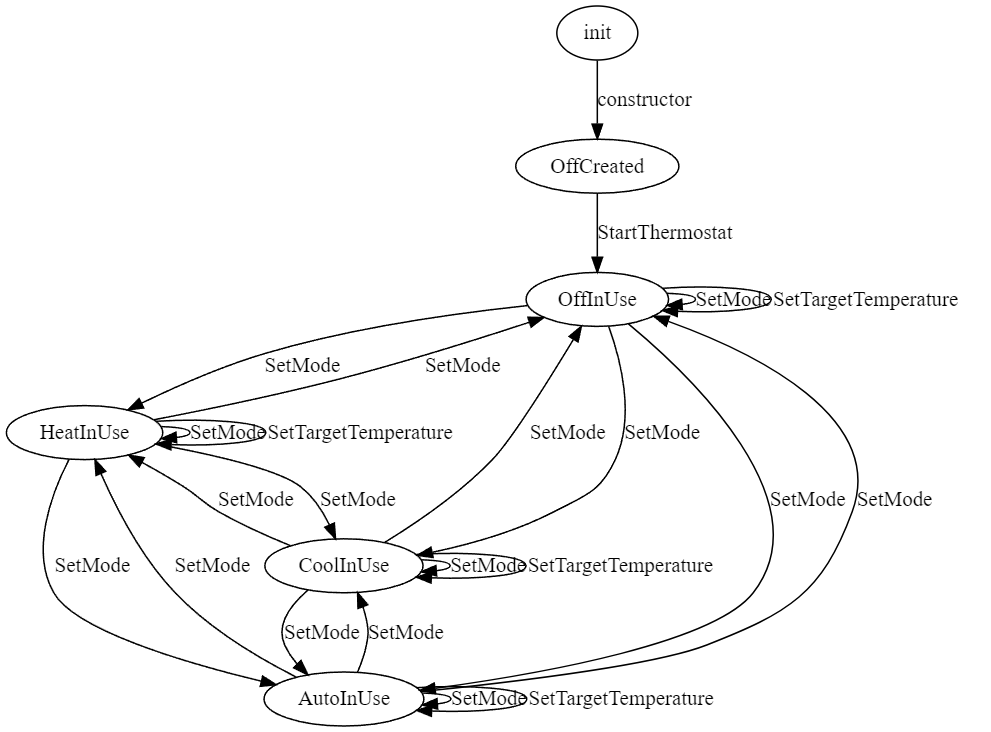
\includegraphics[width=\textwidth]{figs/room-thermostate-abstraction.png}}
    \caption{Abstracción por estado de las variables \textcolor{cyan}{\texttt{enum} del contrato \texttt{RoomThermostat}}}
    \label{fig:room-thermostat-states}
\end{figure}

A la hora de implementar la generación de estas abstracciones, para poder utilizar el mismo mecanismo de generación de abstracciones que el utilizado para las EPAs era necesario conocer el valor de las variables de instancia de tipo \textcolor{cyan}{\texttt{enum}}.
Aquí, nuevamente por consideraciones en el tiempo de desarrollo, lo mas sencillo fue tratar la introspección de estas variables de manera similar a los valores de las precondiciones de los métodos.
Lo que hicimos fue definir métodos externos para cada una de las variables de instancia de tipo \textcolor{cyan}{\texttt{enum}} que permitieran observar el valor de esta variable.
Luego, podíamos detectar estos métodos introduciendo un nuevo tipo sufijo ``\textcolor{orange}{\texttt{\_enum}}''.
Por ejemplo, para la variable \texttt{Mode} en el contrato \texttt{RoomThermostat}, el método generado era el siguiente:

\begin{lstlisting}[language=Solidity]
    function Mode_enum() public returns (ModeEnum) {
        return Mode;
    }
\end{lstlisting}

Utilizando estos nuevos métodos externos el mecanismo para generar las abstracciones era el mismo que el de las EPAs, con la diferencia de que los estados se construían tomando combinaciones de los \textcolor{cyan}{\texttt{enum}} en lugar de de las precondiciones.
